% Timed defence: 22 slides for a 20-minute presentation.

\begin{frame}[plain]\titlepage\end{frame}

\begin{frame}{Outline}\tableofcontents\end{frame}

\renewcommand{\sectionblurb}{What the machine actually does, why the job order changes the cost, and the two questions this work answers.}
\section{The problem}

% ---------------------------------------------------------------- 1 (new)
\begin{frame}{A machine, a magazine, and a set of jobs}
\vspace{0.1cm}
\begingroup\centering
\scalebox{.88}{\begin{tikzpicture}[
   font=\small, >=Stealth,
   job/.style={draw=cBlue!70, fill=white, rounded corners, semithick,
               minimum width=2.7cm, minimum height=1.0cm, align=center},
   chip/.style={draw=black!25, rounded corners=1pt, minimum size=0.72cm,
                inner sep=0pt, font=\bfseries, text=white},
   swaparr/.style={->, line width=1.1pt, cRed}]
  \node[job] (j1) at (0,2)   {\textbf{job 1} needs\\ {\color{cRed}$a$}, {\color{cBlue}$b$}};
  \node[job] (j2) at (5,2)   {\textbf{job 2} needs\\ {\color{cBlue}$b$}, {\color{cGreen}$c$}};
  \node[job] (j3) at (10,2)  {\textbf{job 3} needs\\ {\color{cGreen}$c$}, {\color{cOrange}$d$}};
  \node[chip,fill=cRed]    (m1a) at (-0.42,0) {$a$};
  \node[chip,fill=cBlue]   (m1b) at ( 0.42,0) {$b$};
  \node[chip,fill=cBlue]   (m2a) at ( 4.58,0) {$b$};
  \node[chip,fill=cGreen]  (m2b) at ( 5.42,0) {$c$};
  \node[chip,fill=cGreen]  (m3a) at ( 9.58,0) {$c$};
  \node[chip,fill=cOrange] (m3b) at (10.42,0) {$d$};
  \node[draw=black!45, rounded corners, fit=(m1a)(m1b), inner sep=2.5pt] (m1) {};
  \node[draw=black!45, rounded corners, fit=(m2a)(m2b), inner sep=2.5pt] (m2) {};
  \node[draw=black!45, rounded corners, fit=(m3a)(m3b), inner sep=2.5pt] (m3) {};
  \draw[->,black!45] (j1) -- (m1);  \draw[->,black!45] (j2) -- (m2);  \draw[->,black!45] (j3) -- (m3);
  \draw[swaparr] (m1) -- (m2)
     node[midway,above,font=\scriptsize,align=center]{swap\\ $-a$, $+c$};
  \draw[swaparr] (m2) -- (m3)
     node[midway,above,font=\scriptsize,align=center]{swap\\ $-b$, $+d$};
  \node[font=\scriptsize,text=black!55] at (5,-1.05) {the magazine (the grey box) holds only two tools at a time};
\end{tikzpicture}}
\par\endgroup
\vspace{0.3cm}
\begin{itemize}\itemsep5pt
  \item One machine makes many different parts. Each part --- a \textbf{job} --- needs its
        own small set of tools.
  \item The tools sit in a \textbf{magazine} that holds only a few at a time. To run a job,
        every tool it needs must be in the magazine.
  \item Swapping a tool stops the machine, and each stop costs time. So the thing to
        minimise is the \textbf{number of tool insertions}.
\end{itemize}
\vspace{0.3cm}
\centering
Two decisions: \textbf{the order of the jobs}, and \textbf{what stays loaded}.
\end{frame}

% ---------------------------------------------------------------- 2 (theirs, notation removed)
\begin{frame}{Why the order matters}
\vspace{0.1cm}
\begingroup\centering
\scalebox{1.0}{\begin{tikzpicture}[
   font=\small, >=Stealth,
   slot/.style={draw=black!45, rounded corners=1pt, minimum size=0.62cm,
                inner sep=0pt, font=\small},
   fresh/.style={slot, fill=black!72, text=white, draw=black!72},
   held/.style={slot, fill=black!8},
   jl/.style={font=\scriptsize\bfseries, text=black!75}]

 % ---------------- row 1 : order 1,2,3 -> cost 4 ----------------
 \begin{scope}
   \node[font=\small\bfseries, anchor=west] at (-2.35,1.02) {order $1,2,3$};
   \node[anchor=west, font=\small] at (2.55,1.02) {four tool insertions \textbf{(optimal)}};
   \foreach \x/\lab in {0/{job 1},2.3/{job 2},4.6/{job 3}}
     \node[jl] at (\x+0.31,0.62) {\lab};
   % job1 {a,b}: both new
   \node[fresh] (r1a) at (0,0)    {$a$};  \node[fresh] (r1b) at (0.62,0) {$b$};
   % job2 {b,c}: b held, c new
   \node[held]  (r2b) at (2.3,0)  {$b$};  \node[fresh] (r2c) at (2.92,0) {$c$};
   % job3 {c,d}: c held, d new
   \node[held]  (r3c) at (4.6,0)  {$c$};  \node[fresh] (r3d) at (5.22,0) {$d$};
   \foreach \a/\b in {r1b/r2b, r2c/r3c}
     \draw[->, black!45, shorten >=2pt, shorten <=2pt] (\a) to[bend left=38] (\b);
   \node[font=\scriptsize, text=black!60, anchor=west] at (6.15,0) {$2+1+1=4$};
 \end{scope}

 % ---------------- row 2 : order 1,3,2 -> cost 5 ----------------
 \begin{scope}[yshift=-2.15cm]
   \node[font=\small\bfseries, anchor=west] at (-2.35,1.02) {order $1,3,2$};
   \node[anchor=west, font=\small] at (2.55,1.02) {five --- one insertion wasted};
   \foreach \x/\lab in {0/{job 1},2.3/{job 3},4.6/{job 2}}
     \node[jl] at (\x+0.31,0.62) {\lab};
   \node[fresh] (s1a) at (0,0)    {$a$};  \node[fresh] (s1b) at (0.62,0) {$b$};
   \node[fresh] (s2c) at (2.3,0)  {$c$};  \node[fresh] (s2d) at (2.92,0) {$d$};
   \node[held]  (s3c) at (4.6,0)  {$c$};  \node[fresh] (s3b) at (5.22,0) {$b$};
   \draw[->, black!45, shorten >=2pt, shorten <=2pt] (s2c) to[bend left=38] (s3c);
   \node[font=\scriptsize, text=black!60, anchor=west] at (6.15,0) {$2+2+1=5$};
 \end{scope}

 % ---------------- legend ----------------
 \node[fresh] (lg1) at (-1.6,-3.35) {};
 \node[anchor=west, font=\scriptsize, text=black!65] at (-1.25,-3.35) {inserted here (counted)};
 \node[held]  (lg2) at (2.75,-3.35) {};
 \node[anchor=west, font=\scriptsize, text=black!65] at (3.1,-3.35) {already loaded (free)};
\end{tikzpicture}}
\par\endgroup
\vspace{0.35cm}
Same jobs, same magazine, same loading rule. Only the order changed --- and running job~2
last forces a tool out and then back in.

\vspace{0.32cm}
\centering
That second insertion is a \textbf{reinsertion}, and it is what this whole talk is about.
\end{frame}

% ---------------------------------------------------------------- 3 (theirs, Z* now named here)
\begin{frame}{Schedules as walks through configurations}
\vspace{0.01cm}
\begingroup\centering
\scalebox{.70}{\begin{tikzpicture}[font=\footnotesize,>=Stealth,
   cfg/.style={draw=cPurple!70,semithick,fill=white,rounded corners,minimum width=1.6cm,minimum height=0.85cm},
   bad/.style={draw=cRed!70,semithick,fill=white,rounded corners,minimum width=1.75cm,minimum height=0.85cm},
   node distance=1.15cm]
 \begin{scope}
  \node[font=\footnotesize\bfseries,anchor=west] at (-0.9,1.15)
     {four configurations: cost $3$};
  \node[cfg] (c1) {$\{1,2,3\}$};
  \node[cfg,right=of c1] (c2) {$\{1,3,4\}$};
  \node[cfg,right=of c2] (c3) {$\{1,4,5\}$};
  \node[cfg,right=of c3] (c4) {$\{1,5,6\}$};
  \draw[->,semithick,black!60] (c1)--(c2) node[midway,above,font=\scriptsize]{$+4$};
  \draw[->,semithick,black!60] (c2)--(c3) node[midway,above,font=\scriptsize]{$+5$};
  \draw[->,semithick,black!60] (c3)--(c4) node[midway,above,font=\scriptsize]{$+6$};
  \node[below=0.5mm of c1,font=\scriptsize,text=black!60] {serves $1,2$};
  \node[below=0.5mm of c2,font=\scriptsize,text=black!60] {serves $3$};
  \node[below=0.5mm of c3,font=\scriptsize,text=black!60] {serves $4$};
  \node[below=0.5mm of c4,font=\scriptsize,text=black!60] {serves $5,6$};
 \end{scope}
 \begin{scope}[yshift=-3.2cm]
  \node[font=\footnotesize\bfseries,anchor=west] at (-0.9,1.15)
     {three configurations: cost $4$};
  \node[bad] (a) at (0.6,0) {$\{1,2,3\}$};
  \node[bad] (b) at (3.9,0) {$\{3,4,5\}$};
  \node[bad] (c) at (7.2,0) {$\{5,6,1\}$};
  \draw[->,semithick,black!60] (a)--(b) node[midway,above,font=\scriptsize]{$+4,+5$};
  \draw[->,semithick,black!60] (b)--(c) node[midway,above,font=\scriptsize]{$+6,+1$};
  \node[below=0.5mm of a,font=\scriptsize,text=black!60] {serves $1,2$};
  \node[below=0.5mm of b,font=\scriptsize,text=black!60] {serves $3,4$};
  \node[below=0.5mm of c,font=\scriptsize,text=black!60] {serves $5,6$};
 \end{scope}
\end{tikzpicture}}
\par\endgroup
\vspace{0.15cm}
{\small A \textbf{configuration} is one full magazine. A schedule is a walk from one to the
next, costing the tools that enter along the way. This picture is behind both halves of
the talk.}

\vspace{0.2cm}
\begin{block}{Two quantities, for the rest of the talk}
{\small Write $b$ for the magazine capacity, $T_j$ for the tools job $j$ needs, and $\U$
for the tools the instance actually uses. Let $\Zst$ be the fewest insertions any schedule
achieves. At most $b$ tools are loaded before the first job and every other one must enter
at least once, so $\Zst\ge q:=\lvert\U\rvert-b$ --- an elementary count.}
\end{block}
\end{frame}

\begin{frame}{One decision is easy, the other is not}
\vspace{0.05cm}
\begin{columns}[T,onlytextwidth]
\column{.55\textwidth}
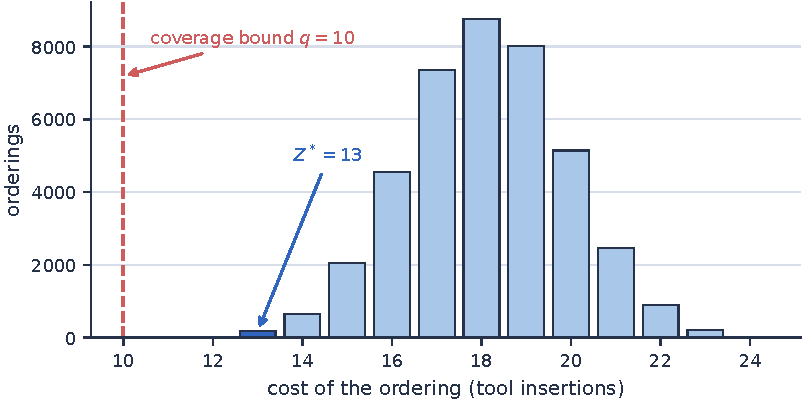
\includegraphics[width=\linewidth,height=.62\textheight,keepaspectratio]{assets/report_figures/landscape.pdf}
\column{.41\textwidth}
\textbf{Once the order is fixed}\\[.12cm]
{\small When a tool must enter a full magazine, remove the one whose next use lies
furthest ahead --- the \emph{Keep Tool Needed Soonest} rule (KTNS). It is optimal, and
it is fast.}\\[.14cm]
{\small{\itshape\color{muted}Tang \& Denardo (1988)}}

\vspace{0.3cm}
\textbf{Choosing the order}\\[.12cm]
{\small NP-hard for every magazine capacity of two or more.}\\[.14cm]
{\small{\itshape\color{muted}Crama et al. (1994)}}
\end{columns}
\vspace{0.24cm}
\begin{columns}[T,onlytextwidth]
\column{.31\textwidth}\centering\keyfig{$40{,}320$}{orders of \texttt{L1-1}, a standard eight-job benchmark}
\column{.31\textwidth}\centering\keyfig{$180$}{of them are optimal}
\column{.31\textwidth}\centering\keyfig{$q=10$ \textit{vs} $\Zst=13$}{the count is three short}
\end{columns}
\end{frame}

% ---------------------------------------------------------------- 4 (new)

% ---------------------------------------------------------------- 5 (theirs, q definition removed)
\begin{frame}{Where the literature stops}
\vspace{0.2cm}
\begin{columns}[T,onlytextwidth]
\column{.47\textwidth}
\textbf{What practice does}\\[.18cm]
Pack jobs into the fewest batches that fit the magazine, then order the batches. Known to
be a $b$-approximation, and it does well in the one industrial study.\\[.22cm]
{\small{\itshape\color{muted}Crama \& van de Klundert (1999); Burger et al. (2015)}}

\vspace{0.28cm}
\textbf{Missing:} an instance-sensitive account of when this construction loses.

\column{.47\textwidth}
\textbf{What exact models do}\\[.18cm]
Four decades of integer models. Of the three reimplemented here, the strongest relaxes to
exactly the elementary count $q$ --- no better than counting.\\[.22cm]
{\small{\itshape\color{muted}Laporte et al. (2004); Catanzaro et al. (2015); da Silva et al. (2021)}}

\vspace{0.28cm}
\textbf{Missing:} a useful certificate when $q$ is not the optimum.
\end{columns}
\end{frame}

% ---------------------------------------------------------------- 6 (theirs)
\begin{frame}{The two questions}
\vspace{0.3cm}
\begin{columns}[T,onlytextwidth]
\column{.46\textwidth}
\textbf{1. Grouping}\\[.2cm]
What does insisting on the \emph{fewest} groups cost, once the order it produces is
reloaded optimally?

\vspace{0.4cm}
\textbf{Answered by:} identities, zero-gap cases, a ratio bound, and a family where the
loss grows without bound.

\column{.46\textwidth}
\textbf{2. Exact optimisation}\\[.2cm]
Can an exact loading oracle carry a solver past the counting bound $q$?

\vspace{0.4cm}
\textbf{Answered by:} a branch-and-Benders-cut solver, four strengthenings, and a campaign
of sixteen thousand runs.
\end{columns}
\vspace{0.5cm}
\centering
Both live on the same walk: one restricts which walks are allowed, the other asks what can
be \emph{proved} about all of them.
\end{frame}

\renewcommand{\sectionblurb}{The heuristic industry uses is better than its published worst cases suggest --- and worse than they can prove.}
\section{Structural results}

\begin{frame}{The standard worst-case example is not a worst case}
\vspace{0.01cm}
\begingroup\centering
\scalebox{.49}{\begin{tikzpicture}[x=0.8cm,y=0.8cm,font=\footnotesize]
 % ---------------- (a) the configuration walk ----------------
 \begin{scope}
  \node[font=\footnotesize\bfseries,anchor=west] at (0.15,7.6)
     {(a) the walk: one magazine per group};
  \foreach \p/\req in {1/{1{,}2},2/{2{,}3},3/{3{,}4},4/{4{,}5},5/{5{,}6},6/{6{,}1}}{
    \node[font=\footnotesize] at (\p,6.05) {\p};
    \node[font=\scriptsize,text=black!55] at (\p,6.7) {$\{\req\}$};}
  \foreach \t/\y in {1/5,2/4,3/3,4/2,5/1,6/0}{
    \node[anchor=east,font=\footnotesize] at (0.4,\y) {$t_{\t}$};}
  \foreach \p/\y in {1/5,2/5,5/5,6/5, 1/4,2/4, 1/3,2/3,3/3,4/3,
                     3/2,4/2, 3/1,4/1,5/1,6/1, 5/0,6/0}{
     \fill[cBlue!20] (\p-0.5,\y-0.5) rectangle (\p+0.5,\y+0.5);}
  \foreach \p/\y in {1/5,1/4,1/3, 3/2,3/1, 5/5,5/0}{
     \fill[cOrange!90] (\p-0.5,\y-0.5) rectangle (\p+0.5,\y+0.5);
     \draw[white,line width=0.9pt] (\p-0.17,\y)--(\p+0.17,\y);
     \draw[white,line width=0.9pt] (\p,\y-0.17)--(\p,\y+0.17);}
  \draw[black!35,step=1] (0.5,-0.5) grid (6.5,5.5);
  \draw[black!55,semithick,dashed] (2.5,-0.5) -- (2.5,5.5);
  \draw[black!55,semithick,dashed] (4.5,-0.5) -- (4.5,5.5);
  \foreach \x/\g in {1.5/1,3.5/2,5.5/3}{
    \node[font=\scriptsize,text=black!55] at (\x,-1.05) {$G_{\g}$};}
  \node[font=\scriptsize,text=black!70,anchor=west] at (0.5,-1.8)
     {seven insertions};
 \end{scope}
 % ---------------- (b) KTNS on the same job order ----------------
 \begin{scope}[xshift=7.7cm]
  \node[font=\footnotesize\bfseries,anchor=west] at (0.15,7.6)
     {(b) KTNS on the same job order};
  \foreach \p/\req in {1/{1{,}2},2/{2{,}3},3/{3{,}4},4/{4{,}5},5/{5{,}6},6/{6{,}1}}{
    \node[font=\footnotesize] at (\p,6.05) {\p};
    \node[font=\scriptsize,text=black!55] at (\p,6.7) {$\{\req\}$};}
  \foreach \t/\y in {1/5,2/4,3/3,4/2,5/1,6/0}{
    \node[anchor=east,font=\footnotesize] at (0.4,\y) {$t_{\t}$};}
  \foreach \p/\y in {1/5,2/5,3/5,4/5,5/5,6/5, 1/4,2/4, 1/3,2/3,3/3,
                     3/2,4/2, 4/1,5/1,6/1, 5/0,6/0}{
     \fill[cBlue!20] (\p-0.5,\y-0.5) rectangle (\p+0.5,\y+0.5);}
  \foreach \p/\y in {1/5,1/4,1/3, 3/2, 4/1, 5/0}{
     \fill[cOrange!90] (\p-0.5,\y-0.5) rectangle (\p+0.5,\y+0.5);
     \draw[white,line width=0.9pt] (\p-0.17,\y)--(\p+0.17,\y);
     \draw[white,line width=0.9pt] (\p,\y-0.17)--(\p,\y+0.17);}
  \draw[black!35,step=1] (0.5,-0.5) grid (6.5,5.5);
  \draw[black!55,semithick,dashed] (2.5,-0.5) -- (2.5,5.5);
  \draw[black!55,semithick,dashed] (4.5,-0.5) -- (4.5,5.5);
  \foreach \x/\g in {1.5/1,3.5/2,5.5/3}{
    \node[font=\scriptsize,text=black!55] at (\x,-1.05) {$G_{\g}$};}
  \node[font=\scriptsize,text=black!70,anchor=west] at (0.5,-1.8)
     {six insertions};
 \end{scope}
\end{tikzpicture}}
\par\endgroup
\vspace{0.2cm}
\begin{columns}[T,onlytextwidth]
\column{.46\textwidth}
\textbf{(a) What the literature draws}\\[.14cm]
One magazine per group, held while that group runs. Every published worst case for this
method is built on this picture. Here it pays \textbf{one extra insertion}.
\column{.46\textwidth}
\textbf{(b) What the method actually does}\\[.14cm]
It reloads the whole job order optimally at the end. On the same instance it pays
\textbf{nothing extra} --- it is optimal.
\end{columns}
\vspace{0.28cm}
\centering
This is \emph{the} example the field reaches for to show this heuristic losing. Under the
method as specified, \textbf{it does not lose.}
\end{frame}


\begin{frame}{So the loss is real --- but you need a different construction}
\vspace{0.06cm}
\begingroup\centering
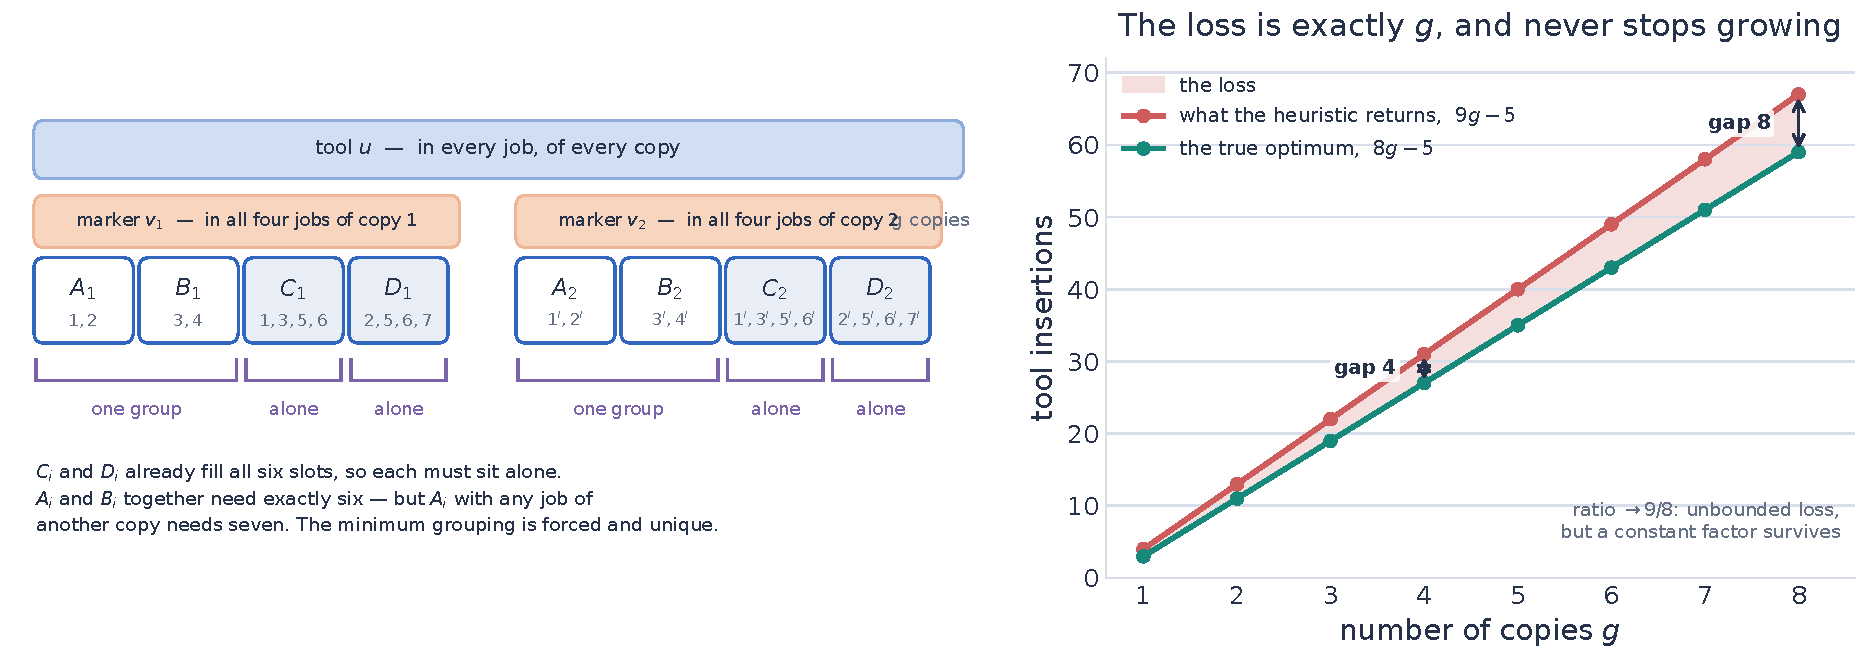
\includegraphics[width=.99\linewidth,height=.56\textheight,keepaspectratio]{assets/defence_figures/unbounded_family.pdf}
\par\endgroup
\vspace{0.22cm}
\begin{columns}[T,onlytextwidth]
\column{.47\textwidth}
{\small Every job shares one tool, so the instance is \textbf{connected} --- this is not
$g$ separate problems placed side by side. The loss is exactly $g$ and grows without
bound.}
\column{.47\textwidth}
{\small And the loss is exactly the price of insisting on the \emph{fewest} groups: allow
every grouping and the construction becomes exact. Nothing else in the method is at
fault.}
\end{columns}
\end{frame}


\renewcommand{\sectionblurb}{Hand the easy half to an exact oracle, and let the hard half be searched. Where the cuts come from, and what they can say.}
\section{A branch-and-Benders-cut algorithm}

\begin{frame}{The decomposition}
\vspace{0.06cm}
\begingroup\centering
\scalebox{.95}{\begin{tikzpicture}[font=\footnotesize,>=Stealth,
   blk/.style={draw,semithick,rounded corners,align=center,minimum height=1.6cm,text width=3.7cm}]
  \node[blk,draw=cBlue!70,fill=white] (m) {\textbf{Master} (hard)\\[2pt] choose the job order,\\ minimising the stand-in $\theta$};
  \node[blk,right=4.2cm of m,draw=cGreen!70,fill=white] (s) {\textbf{Subproblem} (easy)\\[2pt] load the tools for that\\ order, \emph{exactly}};
  \draw[-{Stealth[length=3mm]},semithick,black!60] (m.north east) to[bend left=22] node[above,font=\scriptsize]{an order} (s.north west);
  \draw[-{Stealth[length=3mm]},semithick,black!60] (s.south west) to[bend left=22]
      node[below,align=center,font=\scriptsize,inner sep=2pt]{Benders cut:\\ $\theta\ge$ true cost} (m.south east);
  \node[below=1.28cm of $(m.south)!0.5!(s.south)$,text width=9.4cm,align=center,font=\scriptsize,text=black!60]
     {repeat until $\theta$ equals the loading cost; the order is then a certified optimum};
\end{tikzpicture}
}
\par\endgroup
\vspace{0.19cm}
\begin{enumerate}\itemsep3pt
  \item The master proposes an order and an optimistic loading cost $\theta$.
  \item The subproblem returns the \textbf{exact} loading cost of that order.
  \item A dual solution produces a cut valid for every order and tight at the priced one.
\end{enumerate}
\vspace{0.12cm}
\centering\small
Logic-based and combinatorial Benders lineage:
{\itshape\color{muted}Hooker \& Ottosson (2003); Codato \& Fischetti (2006)}.
\end{frame}

\begin{frame}{The master problem}
\vspace{0.12cm}
Let $d$ be an empty depot and $x_{ij}=1$ when $j$ follows $i$.
\[
\min\ \theta,\qquad
\sum_{i\ne j}x_{ij}=1\ (\forall j),\qquad
\sum_{j\ne i}x_{ij}=1\ (\forall i),
\]
\[
\sum_{i,j\in S}x_{ij}\le |S|-1 \qquad(S\subseteq J).
\]
\vspace{0.08cm}
\textbf{Convention:} theory uses free-initial $q=|\U|-b$; the BBC oracle charges an
empty start, so $\theta\ge|\U|$.

\vspace{0.1cm}
\textbf{Three bound rows, before any cut is generated:}
\[
\underbrace{\theta\ge|\U|}_{\text{coverage}}
\qquad
\underbrace{\theta\ge \sum_{i,j\in J}w_{ij}x_{ij}+\sum_{j\in J}|T_j|x_{dj}}_{\text{pairwise},\ w_{ij}=\max(0,|T_i\cup T_j|-b)}
\qquad
\underbrace{\theta\ge w_{ijk}(x_{ij}+x_{jk}-1)}_{\text{triplet, optional}}
\]
\vspace{-0.1cm}

\centering{\small All three are visible to the root relaxation. Keep that in mind --- the
last part of the talk is about how little they turn out to be worth.}
\end{frame}

\begin{frame}{The subproblem: loading for a fixed order}
\vspace{0.05cm}
Fix $\bar x$. Let $y_{j,t}$ indicate that tool $t$ is loaded at job $j$, and let
$z_{j,t}$ charge its insertion.
{\small
\[
\begin{aligned}
\min\quad & \sum_{j,t}z_{j,t}\\
\text{s.t.}\quad
&y_{j,t}\ge1 && t\in T_j &&(\nu_{jt})\\
&\sum_t y_{j,t}\le b && \forall j &&(\mu_j)\\
&z_{j,t}\ge y_{j,t}-y_{i,t}-(1-\bar x_{ij})
&&\forall i\ne j,t &&(\lambda_{ijt})\\
&z_{j,t}\ge y_{j,t}-(1-\bar x_{dj})
&&\forall j,t &&(\lambda^d_{jt}).
\end{aligned}
\]}
The last row charges the first job because the machine starts empty.
\end{frame}

\begin{frame}{Why the oracle is exact}
\vspace{0.35cm}
\begin{block}{Exact oracle}
Once $\bar x$ fixes a path, the remaining $y,z$ matrix has the consecutive-ones
property and is totally unimodular. Therefore
\[
\min\{\text{loading LP at }\bar x\}=\KTNS(\bar x).
\]
\end{block}
\vspace{0.35cm}
\begin{columns}[T,onlytextwidth]
\column{.46\textwidth}
\textbf{Primal meaning}\\[.12cm]
Every incumbent order is evaluated at its true loading cost.
\column{.46\textwidth}
\textbf{Remaining difficulty}\\[.12cm]
The master must still certify that no better order exists.
\end{columns}
\vspace{0.35cm}
\centering\small
The oracle uses the fixed-order result of {\itshape\color{muted}Tang \& Denardo (1988)}; it is not a heuristic price.
\end{frame}

\begin{frame}{The optimality cut}
\vspace{0.13cm}
For an optimal dual solution
$(\bar\lambda,\bar\lambda^d,\bar\mu,\bar\nu)$:
\[
\boxed{
\theta\ge
\sum_{i\ne j}\sum_t\bar\lambda_{ijt}(x_{ij}-1)
+\sum_j\sum_t\bar\lambda^d_{jt}(x_{dj}-1)
-b\sum_j\bar\mu_j
+\sum_j\sum_{t\in T_j}\bar\nu_{jt}}
\]
\vspace{0.24cm}
\begin{columns}[T,onlytextwidth]
\column{.31\textwidth}
\textbf{Global}\\[.1cm]
Dual feasibility does not depend on the order.
\column{.31\textwidth}
\textbf{Exact locally}\\[.1cm]
At $\bar x$, the cut equals $\KTNS(\bar x)$.
\column{.31\textwidth}
\textbf{Fractional-ready}\\[.1cm]
It is affine in $x$ and can be separated before integrality.
\end{columns}
\end{frame}

\begin{frame}{A defect found and corrected}
\vspace{0.24cm}
\begin{block}{Initial defect}
Omitting
$\sum_{j,t}\bar\lambda^d_{jt}(x_{dj}-1)$ removes a non-positive correction.
The cut can then overestimate orders with other first jobs and remove the true optimum.
\end{block}
\vspace{0.3cm}
\begin{columns}[T,onlytextwidth]
\column{.46\textwidth}
\textbf{Detection}\\[.15cm]
Independent brute-force testing found \textbf{193} violated optimal points.
\column{.46\textwidth}
\textbf{Correction}\\[.15cm]
Restore the depot term, rederive the cut from the implementation, rerun the complete campaign.
\end{columns}
\vspace{0.32cm}
\centering\small
This is why the final validation uses independent enumeration and dynamic programming,
not only agreement with the solver.
\end{frame}

\renewcommand{\sectionblurb}{Four standard accelerations. One aims at the incumbent, three at the bound. Only one of them helps.}
\section{Strengthening the solver}

\begin{frame}{Four strengthenings}
\vspace{0.22cm}
\begin{tabular}{@{}p{.28\linewidth}p{.21\linewidth}p{.39\linewidth}@{}}
\toprule
\textbf{Mechanism} & \textbf{Target} & \textbf{Implementation here}\\
\midrule
Fractional separation & dual bound & price the same cut at fractional $x$\\[3pt]
Root HGS incumbent & primal bound & warm start and initial cut pool\\[3pt]
Conflict-graph row & dual bound & lower-bound the number of groups\\[3pt]
Pareto lifting & cut choice & select a deeper dual optimum\\
\bottomrule
\end{tabular}\par
\vspace{0.26cm}
{\small \textbf{How they were tested.} One switch at a time on a common base, then all three
together, then the base with fractional separation removed --- nine Benders regimes in all,
each validated against brute force before the campaign.
{\itshape\color{muted}Rahmaniani et al. (2017)}}

\vspace{0.2cm}
\centering
Three different targets. \textbf{Watch which kind helps.}
\end{frame}

\begin{frame}{Fractional Benders cuts}
\vspace{0.06cm}
\textbf{Method.} Price the same affine dual cut at a fractional master solution,
before an integral path exists.\par
\vspace{0.08cm}
\begingroup\centering
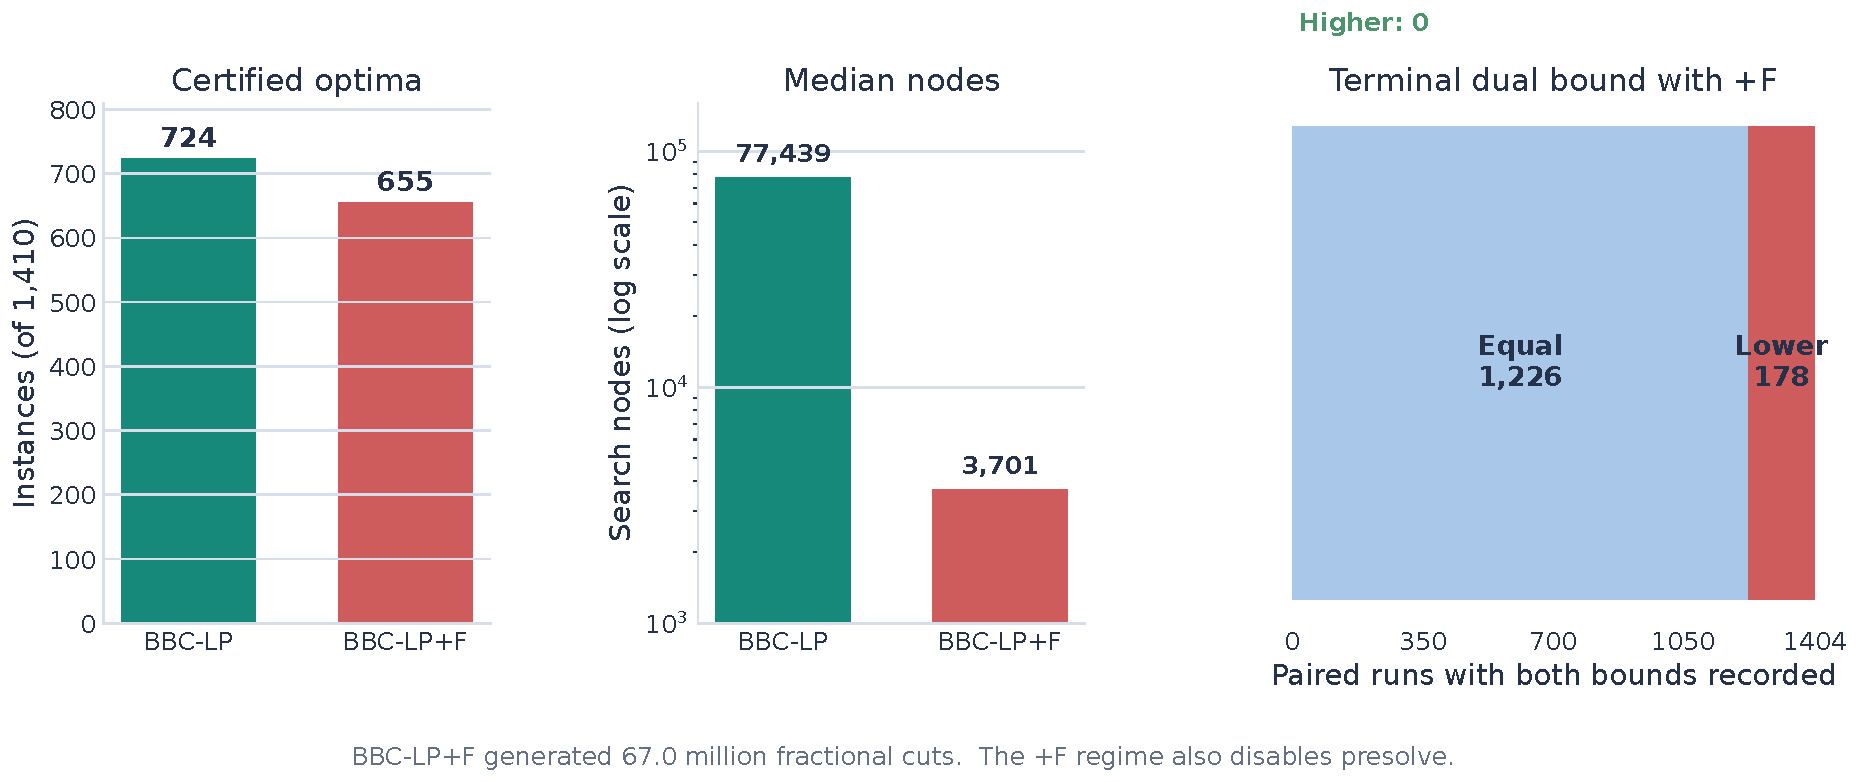
\includegraphics[width=.96\linewidth,height=.47\textheight,keepaspectratio]{assets/defence_figures/fractional_separation_tradeoff.pdf}
\par\endgroup
\vspace{0.14cm}
\begin{columns}[T,onlytextwidth]
\column{.30\textwidth}\centering\keyfig{$67$ million}{cuts generated}
\column{.30\textwidth}\centering\keyfig{$20\times$}{fewer nodes explored}
\column{.34\textwidth}\centering\keyfig{$\mathbf{0}$ of $1{,}404$}{\textbf{terminal bounds improved}}
\end{columns}
\vspace{0.2cm}
\centering
{\small The third number is the finding, and it is the one that is clean. It also loses $69$
certified instances --- but this regime \emph{also} disables presolve, so that figure is
confounded and I do not lean on it. \textbf{Whether these cuts ever raise the bound is not
confounded: they never do.}}
\end{frame}

\begin{frame}{A strong incumbent at the root}
\vspace{0.12cm}
\textbf{Compact HGS at the root} {\itshape\color{muted}Mecler et al. (2021)}:
\[
\begin{gathered}
\text{constructive seeds}\ \longrightarrow\ \text{VNS improvement}\\[-1pt]
\longrightarrow\ \text{order crossover + diversity}
\ \longrightarrow\ \text{exact KTNS scoring}
\end{gathered}
\]
\vspace{0.16cm}
\begin{columns}[T,onlytextwidth]
\column{.46\textwidth}
\textbf{Warm start}\\[.14cm]
The best order supplies an incumbent before branching.
\column{.46\textwidth}
\textbf{Initial cut pool}\\[.14cm]
Its exact loading dual supplies a valid cut before the first relaxation.
\end{columns}
\vspace{0.22cm}
\begin{block}{Measured effect: $+31$ instances --- the only strengthening that gains any}
And it raises the obvious question. Removing fractional separation is worth $+69$; this is
worth $+31$. \textbf{The two were never combined.} That regime is the first thing I would
run next.
\end{block}
\end{frame}

\begin{frame}{The conflict-graph row, and Pareto lifting}
\vspace{0.19cm}
\begin{columns}[T,onlytextwidth]
\column{.47\textwidth}
\textbf{Conflict-graph row}\\[.12cm]
Jobs that cannot share a magazine form edges in $G$. A colouring lower bound gives
\[
\theta\ge(\chi_{\rm lb}-1)+\min(b,|\U|).
\]
It is useful only when grouping structure beats coverage.\\[.13cm]
{\small{\itshape\color{muted}Atamt\"urk et al. (2000)}\\[-1pt]
\textbf{Measured effect: $-1$ instance.}}

\column{.47\textwidth}
\textbf{Pareto-optimal lifting}\\[.12cm]
Among alternative optimal loading duals, maximise the cut value at an interior core
point; retain the ordinary cut as well.\\[.16cm]
{\small{\itshape\color{muted}Magnanti \& Wong (1981); Papadakos (2008)}}\\[.13cm]
\textbf{Measured effect: $-37$ instances.} A deeper cut in the same family is still
arc-supported.
\end{columns}
\end{frame}

\renewcommand{\sectionblurb}{Sixteen thousand runs under one protocol. The compact models win, and the reason is a single quantity.}
\section{Computational results}

\begin{frame}{How far each method gets}
\vspace{0.02cm}
\centering{\small $1{,}410$ instances $\times$ 12 configurations, one hour each. Every
non-optimal outcome counts as unsolved.}

\vspace{0.1cm}
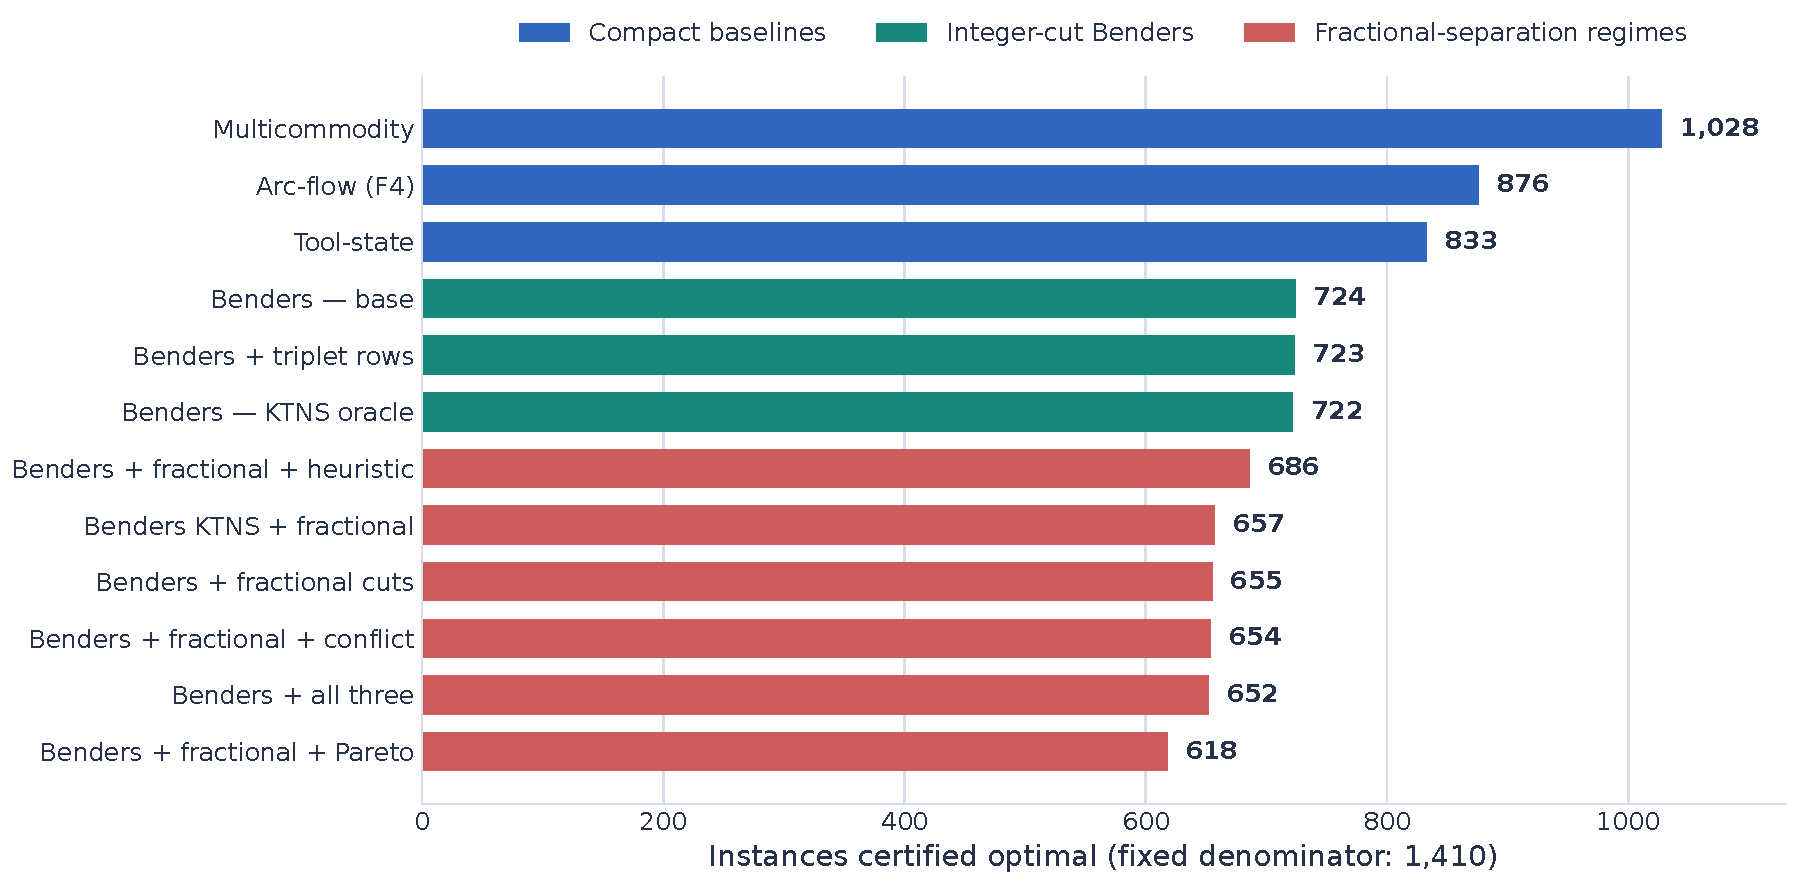
\includegraphics[width=.95\linewidth,height=.60\textheight,keepaspectratio]{assets/defence_figures/solve_counts_all.pdf}

\vspace{0.12cm}
\centering
\textbf{Every compact baseline beats every Benders regime} on the full denominator. But
half that denominator does not discriminate --- and the next slide separates it.
\end{frame}


\begin{frame}{Half the benchmark cannot tell the methods apart}
\vspace{0.3cm}
{\small Laporte3 and Laporte4 are $670$ of the $1{,}410$ instances, and \textbf{all three
compact models close $100\%$ of both}. They are denominator, not evidence. On the $740$
instances that do discriminate:}

\vspace{0.35cm}
\centering
\begin{tabular}{@{}lrr@{}}
\toprule
& \textbf{certified} & \textbf{share}\\
\midrule
Multicommodity                     & $358/740$ & $48.4\%$\\[2pt]
\textbf{Benders + fractional + heuristic} & $\mathbf{213/740}$ & $\mathbf{28.8\%}$\\
Arc-flow (F4)                      & $206/740$ & $27.8\%$\\
Benders --- base                   & $192/740$ & $25.9\%$\\
Tool-state                         & $163/740$ & $22.0\%$\\
\bottomrule
\end{tabular}

\vspace{0.35cm}
\begin{block}{The honest comparison}
On the half of the benchmark where the comparison means anything, this solver is
\textbf{ahead of two of the three baselines} --- while running on one solver thread against
their four. Only the multicommodity model is clearly ahead.
\end{block}
\end{frame}

\begin{frame}{Solving times}
\vspace{0.05cm}
\begingroup\centering
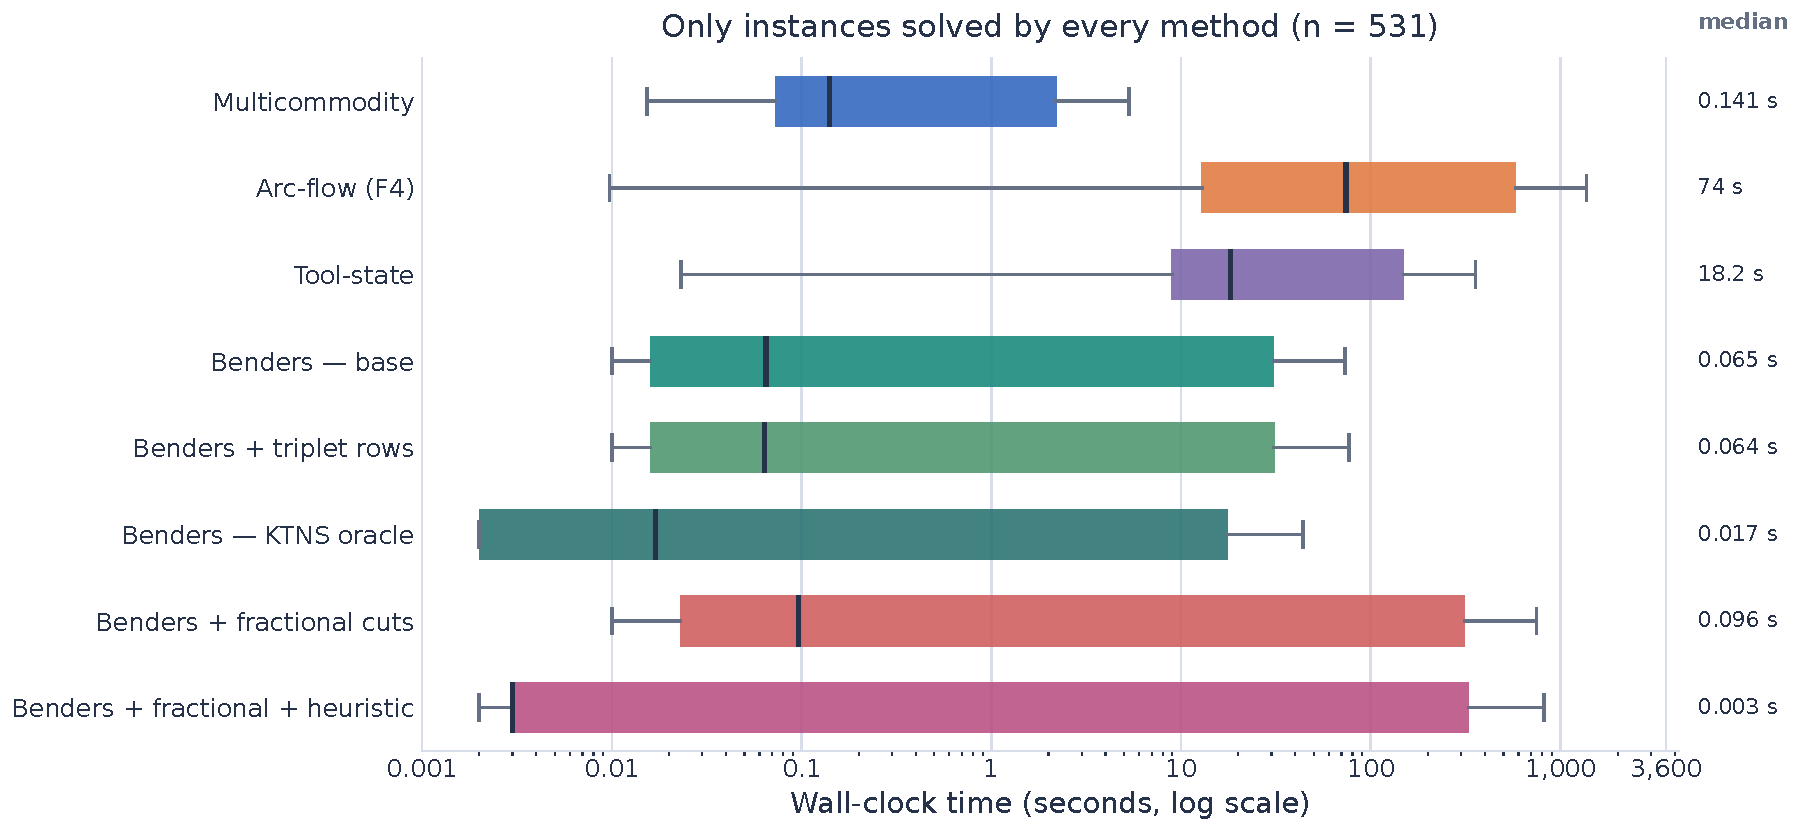
\includegraphics[width=.92\linewidth,height=.64\textheight,keepaspectratio]{assets/defence_figures/common_solved_time_boxplot.pdf}
\par\endgroup
\vspace{0.1cm}
\centering
On the $531$ instances everyone solves, the picture inverts --- the Benders medians sit
orders of magnitude lower. But look at the tails.

\vspace{0.16cm}
\textbf{It closes an instance at once, or not within the hour.} That is the signature of a
bound that is either exactly right or of no use.
\end{frame}

\begin{frame}{What separates the two cases}
\vspace{0.02cm}
\begingroup\centering
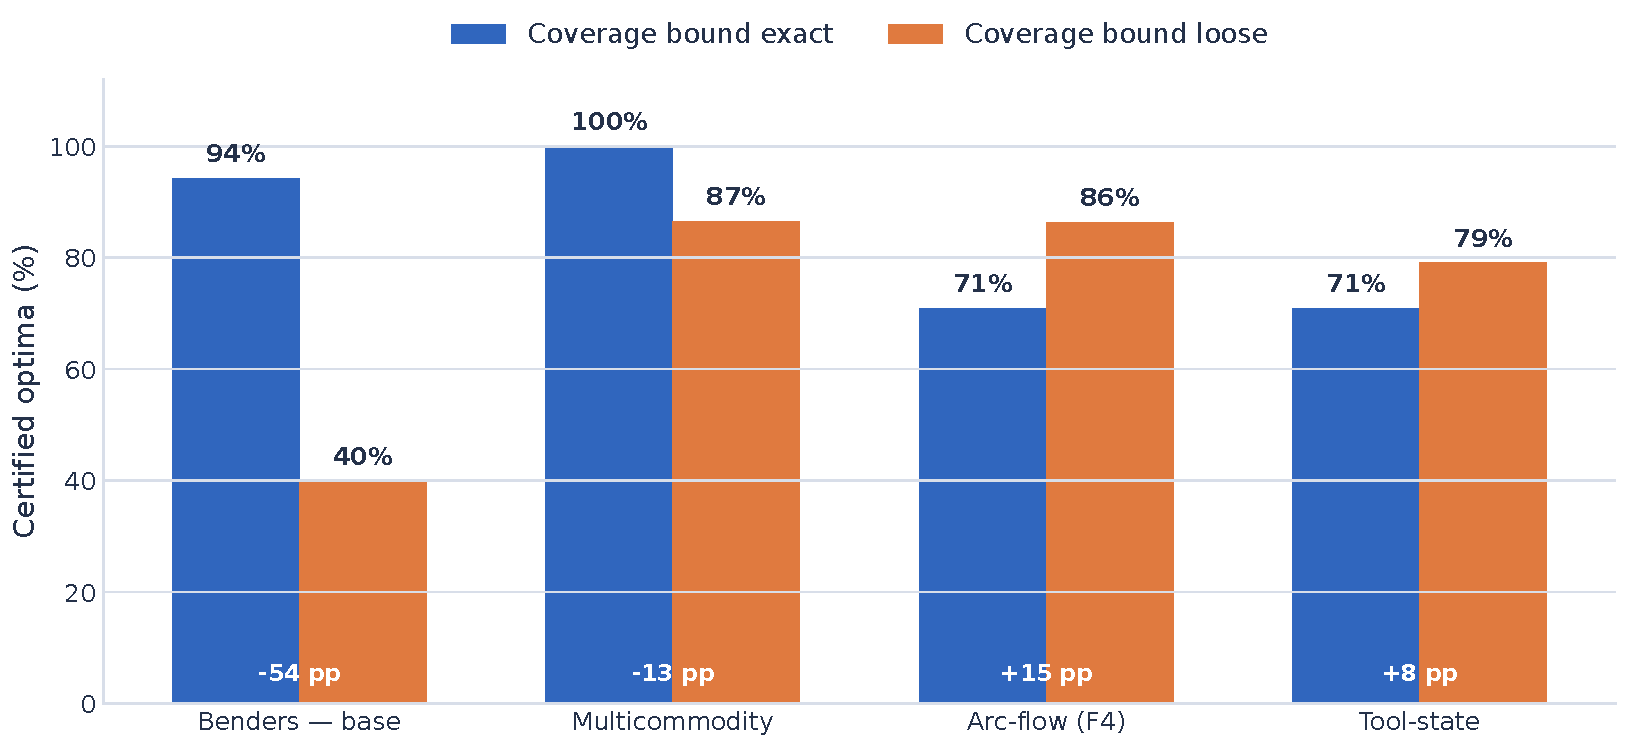
\includegraphics[width=.80\linewidth,height=.46\textheight,keepaspectratio]{assets/defence_figures/coverage_tightness_closure.pdf}
\par\endgroup
\vspace{0.03cm}
\begin{columns}[T,onlytextwidth]
\column{.32\textwidth}\centering
\keyfig{$94\%$ \textit{vs} $40\%$}{closed when $q$ is exact, against when it is loose}
\column{.32\textwidth}\centering
\keyfig{$87\%$}{of roots are the coverage row and nothing more}
\column{.32\textwidth}\centering
\keyfig{$58\%$}{of time-limited runs already hold the optimum}
\end{columns}
\vspace{0.16cm}
\centering
\textbf{But this is a fact about the method, not the instances.} F4 moves the \emph{other}
way and closes every one of the loosest; the multicommodity model, whose relaxation is
also $q$, barely moves
at all. What collapses is a master carrying $q$ and, at the root, little else.
\end{frame}

\renewcommand{\sectionblurb}{Why the bound does not move, what this study does not show, and where the next attempt should go.}
\section{Limitations and conclusions}

\begin{frame}{The cost is not a local quantity}
\vspace{0.01cm}
\small
Recall the counting bound from the start: $q=\lvert\U\rvert-b$ --- one insertion for every
used tool that could not already have been loaded.

\vspace{0.14cm}
Now write $\beta_t$ for the number of separate stretches during which tool $t$ sits in the
magazine. Every insertion of $t$ begins one, so
\[
  \Zst=q+\sum_{t\in\U}(\beta_t-1).
\]
\vspace{-0.22cm}

One stretch per tool gives exactly $q$. \textbf{Everything above $q$ is a reinsertion} --- a
tool evicted and brought back.

\vspace{0.22cm}
A reinsertion happens when the jobs needing a tool are pushed apart by others whose
requirements cannot sit alongside it --- a property of the \textbf{global interleaving} of
the schedule, not of which jobs are adjacent.

\vspace{0.18cm}
\begin{block}{What the master actually carries}
One row indexed by \emph{arcs}, triplet rows that are the weak linearisation of a product,
and a constant coverage row. Every optimality cut it generates is arc-supported too. So it
learns only \textbf{adjacency-indexed} facts about a cost that is not adjacency-indexed.
\end{block}
\end{frame}


\begin{frame}{A family that is not local}
\vspace{0.22cm}
If the diagnosis is right, the fix is an inequality that counts across a \emph{stretch} of
the schedule rather than across one adjacency. So I derived one.

\vspace{0.28cm}
\begin{block}{The window inequality}
Take any block of consecutive positions. Every tool needed somewhere inside that block is
either already loaded when the block begins, or is inserted within it. Counting both sides
bounds the insertions inside the block --- over a \textbf{span}, not an arc.
\end{block}

\vspace{0.28cm}
\begin{columns}[T,onlytextwidth]
\column{.46\textwidth}
\textbf{It looked promising}\\[.12cm]
Screened over integral schedules it had several times the headroom of the rows the solver
already carries.
\column{.46\textwidth}
\textbf{It delivered nothing}\\[.12cm]
It moved \textbf{0 of 37} measured roots --- and then the proof of why: the fractional row
implementing it is \emph{implied} by rows the formulation already has.
\end{columns}
\end{frame}


% ---------------------------------------------------------------- limitations
\begin{frame}{What this study does not show}
\vspace{0.24cm}
\small
\begin{itemize}\itemsep7pt
  \item \textbf{The heuristic census is small.} One fixed census of $1{,}260$ instances at
        three to five jobs. The connected family settles \emph{existence} and
        unboundedness; it says nothing about how often such gaps occur at industrial
        sizes.
  \item \textbf{One hour, one machine, one collection --- and F4, not F5.} Every solve
        count comes from a single limit on one node type, and the compact baseline is
        weaker than the best available. Both points run \emph{against} the conclusion
        drawn here, not for it.
  \item \textbf{The best-looking combination was never run.} Every strengthening was tested
        on top of fractional separation. But removing fractional separation is worth $+69$
        instances and the root heuristic is worth $+31$, so the obvious configuration ---
        the heuristic \emph{without} fractional cuts --- is missing from the campaign. It
        should have been the tenth regime.
\end{itemize}
\end{frame}

\begin{frame}{Conclusions}
\vspace{0.13cm}
\begin{columns}[T,onlytextwidth]
\column{.47\textwidth}
\textbf{Established}\\[.12cm]
{\small
\begin{itemize}\itemsep3pt
  \item Grouping has distinct walk and KTNS-postprocessed values.
  \item Minimum cardinality is exactly the restriction behind the walk gap.
  \item The specified heuristic has an unbounded additive gap on a connected family.
  \item The tested Benders method usually finds good orders but often cannot certify them.
  \item On the discriminating half of the benchmark it is competitive with two of the
        three baselines, at a quarter of their solver threads.
\end{itemize}}

\column{.47\textwidth}
\textbf{Next tests}\\[.12cm]
{\small
\begin{itemize}\itemsep3pt
  \item Run the heuristic \emph{without} fractional separation --- the missing regime.
  \item Price tool residency over spans, not only adjacent arcs.
  \item Disaggregate $\theta$ by position and chain PTF configurations.
  \item Find the exact worst ratio, the strongest $\Kst$-dependent bound, and when
        KTNS closes the walk gap.
  \item Test weighted tool costs and learned column selection.
\end{itemize}}
\end{columns}
\vspace{0.23cm}
\centering
\textbf{The missing object is a useful fractional certificate for non-local tool returns.}

\end{frame}


% ---------------------------------------------------------------- thank you
\begin{frame}[plain]
\vfill
\begingroup\centering
{\Huge\color{navy}\bfseries Thank you}\\[1.0cm]
{\large\color{muted} Questions welcome}
\par\endgroup
\vfill
\end{frame}
